\subsection{Sintonias}
Conforme um elétron completa uma revolução dentro do anel de armazenamento em uma coordenada qualquer $s_0$, sua oscilação de fase $(\varphi - \vartheta)$ avança de
\begin{align}
	\int\limits_{s_0}^{s_0+L}\frac{ds}{\beta}
\end{align}

Devido à periodicidade de $\beta$, esta integral tem o mesmo valor para qualquer $s_0$. Ou seja, em uma revolução completa, a fase da trajetória do elétron é aumentada sempre do mesmo valor. Esse avanço de fase é um fator importante do anel de armazenamento, e é escrito normalmente como $2\pi \nu$, e $\nu$ é chamado de número betatron ou sintonia da máquina. Sua definição é
\begin{align}
	\nu = \frac{1}{2 \pi}\int\limits_{s}^{s+L}\frac{d\bar{s}}{\beta} = \frac{1}{2 \pi}\int\limits_{0}^{L}\frac{ds}{\beta} = \frac{1}{2\pi}\oint \frac{ds}{\beta}\label{eq:2.60}
\end{align}

(O símbolo $\oint$ irá indicar qualquer integração ao redor de todo o anel).
A sintonia é um parâmetro global da máquina, ou seja, não depende da coordenada $s$: ela é a mesma para todo o anel.

As sintonias das coordenadas $x$ e $z$ -- indicadas por $\nu_x$ e $\nu_z$ -- são geralmente diferentes, sendo derivadas das duas funções betatron $\beta_x$ e $\beta_z$. Tanto $\nu_x$ quanto $\nu_z$ são, tipicamente, números não muito grandes próximos de, mas não exatamente, um quarto de inteiro (2.78 ou 5.15, por exemplo). 

Apesar da trajetória betatron ser uma oscilação contorcida não-periódica, se observar uma coordenada fixa ao longo de sucessivas revoluções de um elétron, pode-se concluir que este desvio segue uma forma senoidal. Suponha que esta coordenada fixa é $s_0$ e as sucessivas passagens do elétron sejam indexadas por $j=0,1,2,3,\ ...$. Também considere $\varphi_0$ a fase na passagem 0. Nas passagens seguintes, a fase do movimento irá aumentar de $2\pi\nu$ e, na j-ésima passagem, a fase será
\begin{align}
	2\pi\nu j+ \varphi_0
\end{align}
e o desvio será
\begin{align}
	x_j = a\sqrt{\beta_0}\ cos(2\pi\nu j+ \varphi_0)\label{eq:2.61}
\end{align}
onde $\beta_0$ é o valor da função $\beta$ na coordenada $s_0$.

A amplitude $a\sqrt{\beta_0}$ é constante, então o desvio, avaliado a cada revolução, varia simplesmente como uma simples oscilação senoidal. Como o tempo de cada revolução é constante (desprezando uma pequena correção proporcional a $x$), dado por $\frac{L}{c}$, pode-se descrever o tempo $t_j$ da j-ésima passagem como
\begin{align}
	t_j = \frac{L}{c}j
\end{align}
ou que
\begin{align}
	2\pi j = \omega_r t_j
\end{align}
onde
\begin{align}
	\omega_r = 2\pi \frac{c}{L}
\end{align}
é a frequência angular de revolução do elétron. Então a equação \eqref{eq:2.61} pode ser reescrita, para qualquer $s$ fixo, como
\begin{align}
	x_s (t_j) = a\sqrt{\beta(s)}\ cos(\nu \omega_r t_j + \varphi_{0s})\label{eq:2.64}
\end{align}

\begin{proof}
	Pela equação \eqref{eq:2.48}, $s = s_0 + ct$. Logo, em uma revolução,
	\begin{align*}
		s-s_0 &= ct\\
		L &= ct\\
		\therefore t &= \frac{L}{c}
	\end{align*}
	
	Para a j-ésima revolução,
	\begin{align*}
		t_j = \frac{L}{c}j
	\end{align*}
	
	Isolando $j$,
	\begin{align*}
		j &= \frac{c}{L} t_j\\
		\therefore 2\pi j &= 2\pi \frac{c}{L} t_j
	\end{align*}
	
	Definindo $\omega_r = 2\pi \frac{c}{L}$, então
	\begin{align*}
		2\pi j = \omega_r t_j
	\end{align*}
	e, substituindo isto na equação \eqref{eq:2.61}, tem-se
	\begin{align*}
		x_j = a\sqrt{\beta_0}\ cos(\nu \omega_r t_j + \varphi_{0})
	\end{align*}
	
	Considerando o caso de qualquer coordenada $s$,
	\begin{align*}
		x_s (t_j) = a\sqrt{\beta(s)}\ cos(\nu \omega_r t_j + \varphi_{0s})
	\end{align*}
\end{proof}

Quando uma coordenada $s$ em particular é observada, o movimento lateral é indistinguível de uma simples oscilação harmônica na frequência $\nu \omega_r$ -- normalmente chamada de frequência betatron.

Observando a equação \eqref{eq:2.61}, pode-se ver a justificativa para a afirmativa feita na Seção anterior de que, em cada coordenada longitudinal, deve-se esperar que em algum momento $x$ assumirá seu valor máximo $X(s) = a\sqrt{\beta(s)}$. A menos que $\nu$ seja um número inteiro ou, ainda mais genérico, a não ser que a diferença entre $\nu$ e um inteiro seja uma fração simples -- o que torna a não ser exatamente verdade em um anel de armazenamento real -- a fase (de módulo $2\pi$) em sucessivas passagens de qualquer ponto fixo irá passar por um grande número de valores entre $0$ e $2\pi$ antes de se repetir. E o deslocamento irá em algum momento atingir seu valor de pico $X$ em cada coordenada.

O significado mais importante da sintonia $\nu$ da máquina é relacionado com a existência de ressonâncias que aparecem se $\nu$ assume certos valores. Por exemplo, se $\nu$ é um inteiro, a oscilação betatron iria, idealmente, tornar-se ligeiramente periódica -- repetindo-se a cada revolução. Entretanto, a menor imperfeição no campo guia irá agir como uma perturbação, a qual é síncrona com a frequência de oscilação. Uma pertubação síncrona leva a uma excitação ressonante da oscilação e a um crescimento exponencial da amplitude. Não haverá oscilação estável. Mais adiante será mostrado que outras ressonâncias ocorrem também quando $\nu$ é metade de um inteiro e, se efeitos não-lineares forem considerados, quando a diferença entre $\nu$ e um inteiro é qualquer fração simples.

Ressonâncias devem ser, claro, evitadas nas oscilações betatron radial e vertical. Tem-se que ressonâncias de algum tipo podem ocorrer quando $\nu_x$ e $\nu_z$ satisfazem
\begin{align}
	m \nu_x + n \nu_z = r\label{eq:2.65}
\end{align}
onde $m$, $n$ e $r$ são inteiros. Efeitos significativos são geralmente observados apenas em ressonâncias de ordem baixa, ou seja, estas em que $m$, $n$ e $r$ possuem valores baixos entre 0,1,2,3. O ponto de operação de um anel de armazenamento é especificado por $\nu_x$ e $\nu_z$ e deve ser escolhido de forma a evitar ressonâncias. A relação de ressonância \eqref{eq:2.65} define um conjunto de linhas em um diagrama $\nu_x$, $\nu_z$. Algumas delas estão representadas na \autoref{fig:fig14}, onde um possível ponto de operação também é indicado.

\begin{figure}[!htb]
	\centering
	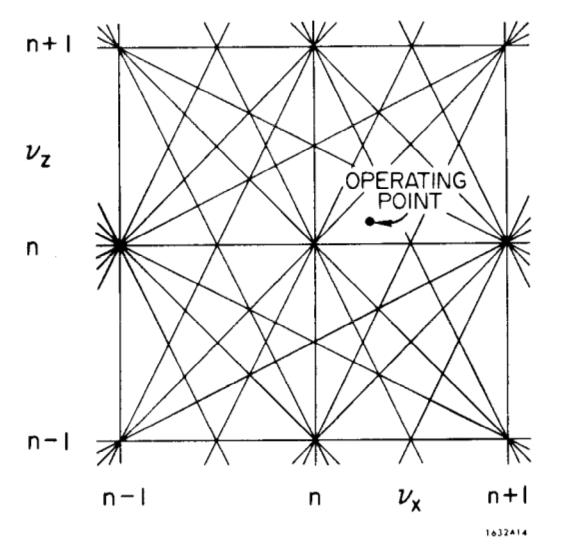
\includegraphics[width=0.6\linewidth]{./Figuras/fig14.jpeg}
	\caption{Ressonâncias de ordem baixa em um diagrama $\nu_x$, $\nu_z$. Retirado de \cite{sands1970physics}.}
	\label{fig:fig14}
\end{figure}

Para um grupo particular de ressonâncias onde $\nu_x$ é igual a $\nu_z$ ou a diferença entre eles é um inteiro, haverá um forte acoplamento entre as oscilações horizontal e vertical. Nesta ressonância, a suposição de que as oscilações são completamente independentes não é mais válida e a modelagem do movimento dos elétrons fica mais complicada. Às vezes, um anel de armazenamento pode ser intencionalmente operadora em uma, ou perto de uma, ressonância de acoplamento a fim de aumentar a amplitude de oscilação vertical alimentando-a com a energia vinda da oscilação radial.

Para estar seguro de ressonâncias perigosas, é preciso que o ponto de operação real esteja perto o suficiente do ponto projetado -- como pode-se ver na \autoref{fig:fig14}. Espera-se que as imperfeições dos ímãs irão causar mudanças em $\nu$ proporcionais ao próprio $\nu$. Um anel de armazenamento com uma sintonia grande é propensa a ser uma máquina "sensível". Por este fato, a sintonia normalmente é escolhida entre valores de 2 a 6.